\documentclass[aspectratio=169]{beamer}
\usepackage[utf8]{inputenc}
\usepackage{amsmath, amssymb}
\usepackage{tikz}
\usetikzlibrary{positioning}
\setbeamertemplate{navigation symbols}{} 

\title{}
\author{{\LARGE Suzie Brown}}
\date{2 November 2018} 

\begin{document}

\begin{frame}
\maketitle
\end{frame}

\begin{frame}
\begin{columns}
\begin{column}{0.4\textwidth}
{\LARGE Genealogies of Sequential Monte Carlo Algorithms}
\end{column}
\begin{column}{0.2\textwidth}
\centering
\includegraphics[width=\textwidth]{jere.jpg}\\
Jere Koskela
\end{column}
\begin{column}{0.2\textwidth}
\centering
\includegraphics[width=\textwidth]{adam.jpg}\\
Adam Johansen
\end{column}
\begin{column}{0.2\textwidth}
\centering
\includegraphics[width=\textwidth]{paul.png}\\
Paul Jenkins
\end{column}
\end{columns}
\end{frame}

\begin{frame}{Hidden Markov model}
\begin{center}
\begin{tikzpicture}
\node (yt) {$Y_t$};
\node (thet) [below=of yt] {$X_t$};
\node (yt1) [left=of yt] {$Y_{t-1}$};
\node (thet1) [below=of yt1] {$X_{t-1}$};
\node (dot1) [left=of thet1] {$\dots$};
\node (dot2) [right=of thet] {$\dots$};
\draw[->](thet.north)--(yt.south) node[left, midway, color=blue] {$g$};
\draw[->](thet1.north)--(yt1.south) node[left, midway, color=blue] {$g$};
\draw[->](thet1.east)--(thet.west) node[below, midway, color=blue] {$f$};
\draw[->](dot1.east)--(thet1.west) node[below, midway, color=blue] {$f$};
\draw[->](thet.east)--(dot2.west) node[below, midway, color=blue] {$f$};
\end{tikzpicture}
\end{center}

\begin{itemize}
\item $\{X_1, X_2, \dots\}$ hidden Markov states
\item $Y_i$ noisy observation of $X_i$
\item Markov transition kernel $f$
\item `emission distribution' $g$
\end{itemize}
% e.g. target tracking: X=true position (and velocity?), Y=observed position
\end{frame}

\begin{frame}{Inference on a HMM}
% at time T:
\begin{itemize}
\item \textbf{filtering distribution} $p(x_{T}\mid y_{1:T})$\\
`current state'
\item \textbf{smoothing distribution} $p(x_{1:T} \mid y_{1:T})$\\
`trajectory of all previous states'
\end{itemize}
\end{frame}

\begin{frame}{Sequential Monte Carlo}
\begin{itemize}
\item Approximate these distributions using $N$ particles
\item  Initialise, then iterate the steps:
\begin{enumerate}
\item \textbf{propagate:} update positions of particles by applying the Markov kernel $f$
\item \textbf{calculate weights:} weight the particles according to how well they agree with the observations
\item \textbf{resample} resample particles proportionally to their weights\\
(`good' particles multiply, `bad' particles die out)
\end{enumerate}
\end{itemize}
\end{frame}

\begin{frame}{Genealogical interpretation}
\begin{itemize}
\item Resampling step induces a genealogical (family tree) structure
%\item (Under some conditions) we can ignore the positions of the particles
\item \textbf{Ancestral degeneracy:} genealogies of all current particles necessarily coalesce at some past time step
\item Bad news for estimating smoothing distribution!
\end{itemize}
% make a beautiful plot to put here, maybe animated
\end{frame}

\begin{frame}{Genealogical interpretation}
\begin{center}
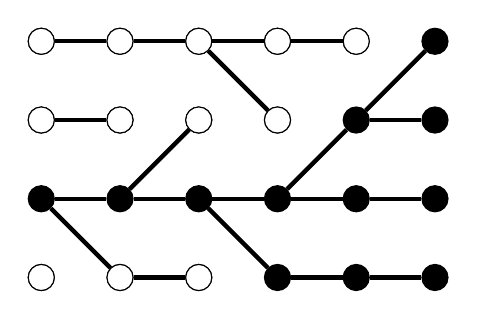
\begin{tikzpicture}
\node[circle, draw=black, fill=black] at (0,3) (11) {};
\node[circle, draw=black, fill=black] at (0,2) (12) {};
\node[circle, draw=black, fill=black] at (0,1) (13) {};
\node[circle, draw=black, fill=black] at (0,0) (14) {};
\pause 

\node[circle, draw=black, fill=black] at (1,3) (21) {};
\node[circle, draw=black, fill=black] at (1,2) (22) {};
\node[circle, draw=black, fill=black] at (1,1) (23) {};
\node[circle, draw=black, fill=black] at (1,0) (24) {};
\draw[ultra thick] (11) -- (21);
\draw[ultra thick] (12) -- (22);
\draw[ultra thick] (13) -- (23);
\draw[ultra thick] (13) -- (24);
\node[circle, draw=black, fill=white] at (0,0) {};
\pause

\node[circle, draw=black, fill=black] at (2,3) (31) {};
\node[circle, draw=black, fill=black] at (2,2) (32) {};
\node[circle, draw=black, fill=black] at (2,1) (33) {};
\node[circle, draw=black, fill=black] at (2,0) (34) {};
\draw[ultra thick] (21) -- (31);
\draw[ultra thick] (23) -- (32);
\draw[ultra thick] (23) -- (33);
\draw[ultra thick] (24) -- (34);
\node[circle, draw=black, fill=white] at (1,2) {};
\node[circle, draw=black, fill=white] at (0,2) {};
\pause

\node[circle, draw=black, fill=black] at (3,3) (41) {};
\node[circle, draw=black, fill=black] at (3,2) (42) {};
\node[circle, draw=black, fill=black] at (3,1) (43) {};
\node[circle, draw=black, fill=black] at (3,0) (44) {};
\draw[ultra thick] (31) -- (41);
\draw[ultra thick] (31) -- (42);
\draw[ultra thick] (33) -- (43);
\draw[ultra thick] (33) -- (44);
\node[circle, draw=black, fill=white] at (2,2) {};
\node[circle, draw=black, fill=white] at (2,0) {};
\node[circle, draw=black, fill=white] at (1,0) {};
\pause

\node[circle, draw=black, fill=black] at (4,3) (51) {};
\node[circle, draw=black, fill=black] at (4,2) (52) {};
\node[circle, draw=black, fill=black] at (4,1) (53) {};
\node[circle, draw=black, fill=black] at (4,0) (54) {};
\draw[ultra thick] (41) -- (51);
\draw[ultra thick] (43) -- (52);
\draw[ultra thick] (43) -- (53);
\draw[ultra thick] (44) -- (54);
\node[circle, draw=black, fill=white] at (3,2) {};
\pause

\node[circle, draw=black, fill=black] at (5,3) (61) {};
\node[circle, draw=black, fill=black] at (5,2) (62) {};
\node[circle, draw=black, fill=black] at (5,1) (63) {};
\node[circle, draw=black, fill=black] at (5,0) (64) {};
\draw[ultra thick] (52) -- (61);
\draw[ultra thick] (52) -- (62);
\draw[ultra thick] (53) -- (63);
\draw[ultra thick] (54) -- (64);
\node[circle, draw=black, fill=white] at (4,3) {};
\node[circle, draw=black, fill=white] at (3,3) {};
\node[circle, draw=black, fill=white] at (2,3) {};
\node[circle, draw=black, fill=white] at (1,3) {};
\node[circle, draw=black, fill=white] at (0,3) {};
\end{tikzpicture}
\end{center}
\end{frame}

\begin{frame}{Genealogical interpretation}
\begin{itemize}
\item How many particles do I need to ensure $n$ distinct lineages remain in generation $T- t$ with probability greater than $1-\alpha$ ?
\pause
\item Easiest case (multinomial resampling) addressed in\\
{\footnotesize Koskela, Jere, et al. "Asymptotic genealogies of interacting particle systems with an application to sequential Monte Carlo." arXiv preprint arXiv:1804.01811 (2018).}
\item \textbf{Next:} relax assumptions, generalise to other resampling schemes and\\ conditional SMC
\end{itemize}
\end{frame}

\end{document}